%%%%%%%%%%%%%%%%%%%%%%%%%%%%%%%%%%%%%%%%%%%%%%%%%%%%%%%%%%%%
%% Chapter 6 - Control Framework and Simulation Integration
%% (12-18 pages)
%% Purpose: specify the complete controller and present the THREE
%% control stacks as one controlled experiment rather than a
%% collection of disconnected models.
%% Main output: reproducible control architecture, policy task
%% definition, integration details, and the matching rules that make
%% the three-way comparison fair.
%%
%% NOTE ON NOMENCLATURE: the only stack names are PPO-ROM (R),
%% PPO-ID-FD (IF) and Adaptive Forward (AF). The earlier PPO1/PPO2 and
%% PPO1-A/B, PPO2-A/B/C/D labels are superseded and must not reappear,
%% and neither must AF or PPO-(AAM)-ID-FD.
%% The BASE policy is NOT a residual policy: it emits its command
%% directly and no nominal command is added at runtime. AF adds a
%% bounded term around that frozen base, but this is an online
%% adaptation mechanism internal to the RL policy, NOT residual RL in
%% the sense of correcting a classical controller: no analytic
%% controller runs underneath at deployment.
%%%%%%%%%%%%%%%%%%%%%%%%%%%%%%%%%%%%%%%%%%%%%%%%%%%%%%%%%%%%
\chapter{Control Framework and Simulation Integration}
\label{chap:control}

Chapter~\ref{chap:models} left three actuator representations, each with its own
contract and offline evidence. This chapter puts a controller in front of them
and turns them into three experiments.

Section~\ref{sec:ctrl:dls} describes the classical controller, because it is
where the competence comes from even though it never runs at deployment.
Section~\ref{sec:ctrl:ppo} specifies the policy: what it sees, what it emits,
what stops it from emitting something dangerous, and what it is paid for.
Section~\ref{sec:ctrl:training} explains how the first becomes the second, and
reports a result about that transfer which changed the training protocol of this
thesis. The individual stacks appear only after those three are fixed.

\section{The DLS Teacher and Its Two Roles}
\label{sec:ctrl:dls}

\subsection{Scope and Role of the Controller}

No damped-least-squares layer runs underneath the policy at runtime and
nothing is added to the policy's output; if the policy emits zero, the arm does
not move. The DLS controller is nevertheless the reason the policies work at
all, and it appears twice, both times at training or collection time and never
at deployment (Figure~\ref{fig:ctrl:teacher-student}). It is the
\emph{privileged teacher} whose behaviour the policies are distilled from
(Section~\ref{sec:ctrl:training}), and it is the closed-loop controller that
drove the identification runs of Section~\ref{sec:data:isaaclab}. Calling it a
nominal layer would misdescribe the deployed system and would make every
reported result a property of a controller pair rather than of the policy.

\begin{figure}[tb]
  \centering
  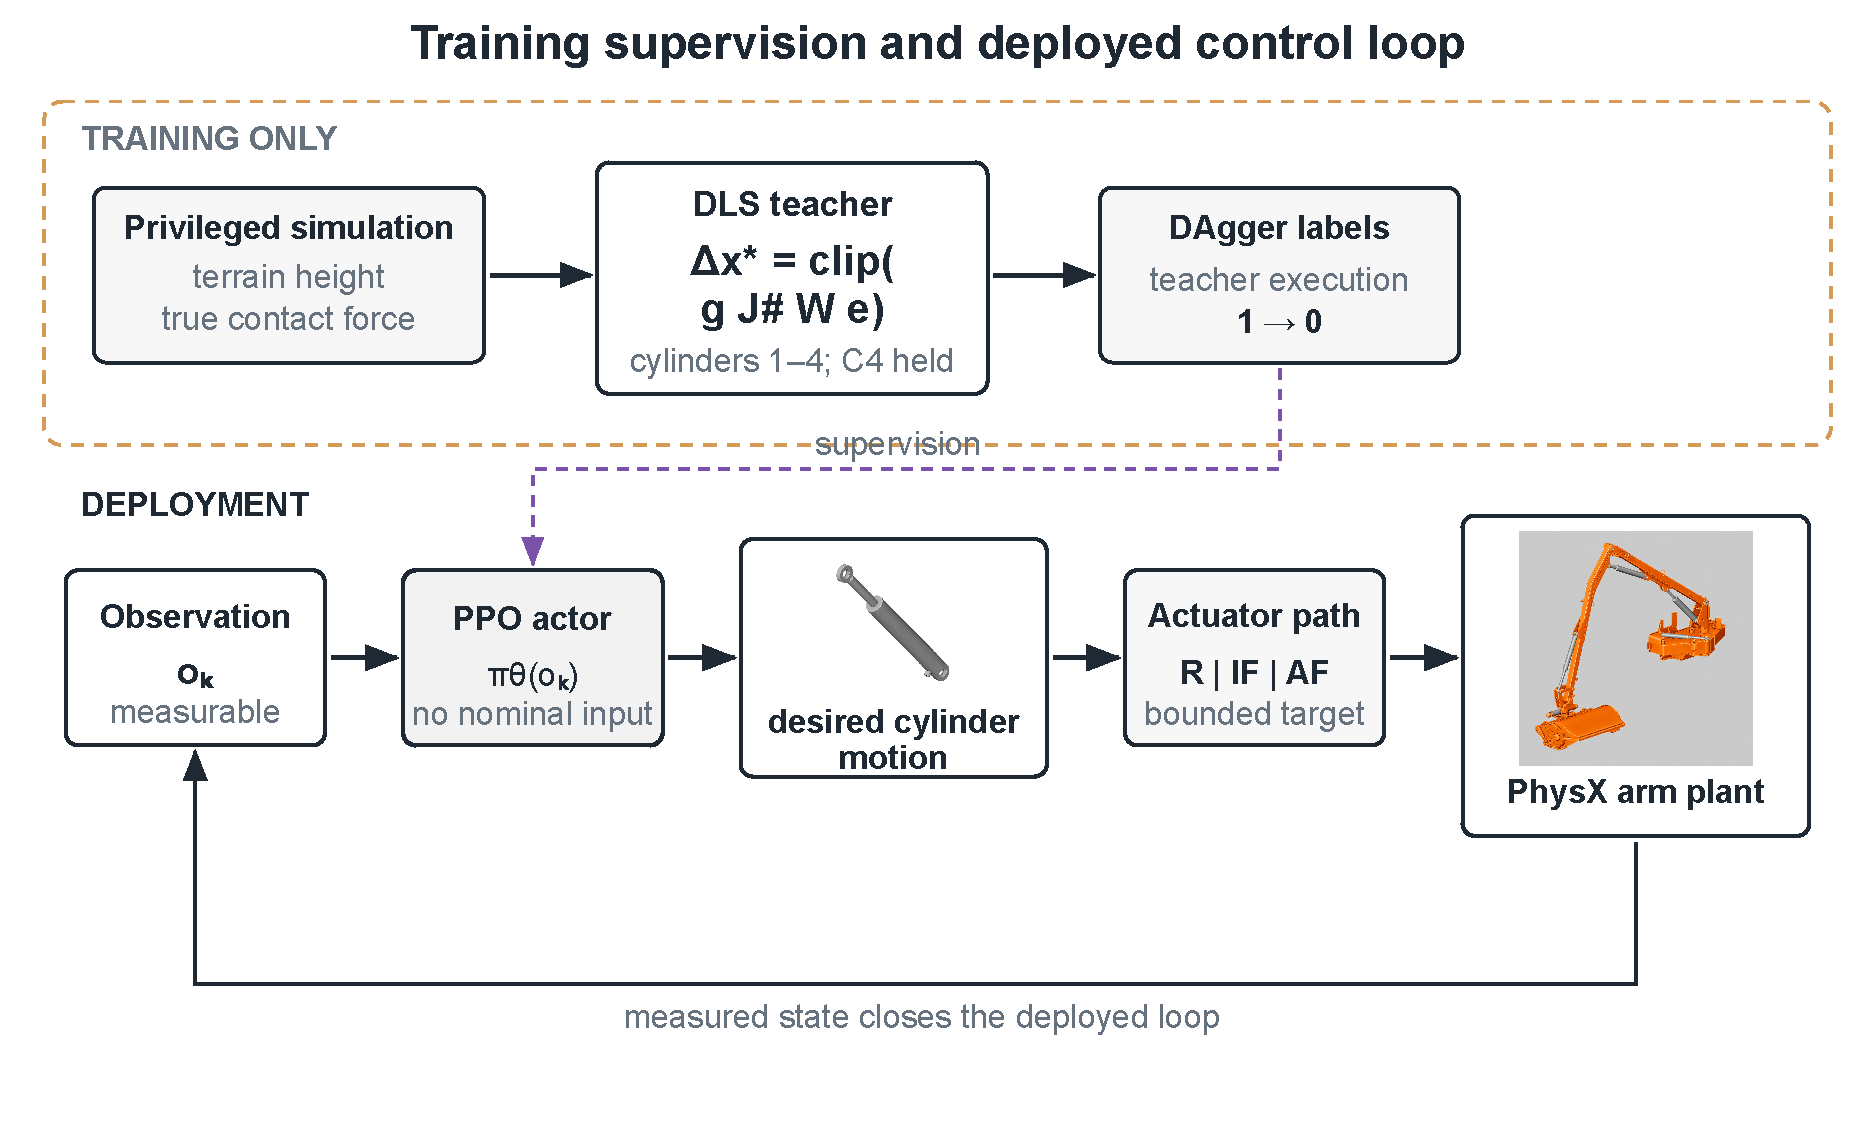
\includegraphics[width=\textwidth]{images/ch6/ch6_teacher_student}
  \caption{Training supervision and deployment. Simulator-only terrain and
  contact signals drive the DLS teacher, which supplies DAgger labels to the
  actor. At deployment only the lower feedback loop remains: measured
  observations pass through the PPO actor, the shared cylinder interface and
  the selected R, IF or AF actuator path before PhysX updates the arm. No
  nominal command is added to the policy output.}
  \label{fig:ctrl:teacher-student}
\end{figure}

\subsection{Privileged Information}

The teacher is \emph{privileged} rather than better tuned: it reads two
quantities that no deployable controller on this machine could obtain, namely
the exact terrain height directly under the cutter, queried from the simulator
rather than inferred from a forward-looking scan, and the true cutter--ground
contact force. Together these turn the hardest part of the task, knowing where
the ground is underneath a $\unit[1.2]{m}$ flail head that is occluding it,
into a lookup.

The teacher uses that privilege in a specific way. Rather than commanding a
height, it runs a contact regulator: it maintains a vertical offset relative to
the ground and adjusts that offset to hold the measured contact force near
$\unit[250]{N}$ within a $\unit[100]{N}$ deadband, pressing down below the band,
backing off proportionally above it, searching downward when contact is lost
and retreating immediately on a force spike. The accumulated offset is clamped
to $[-0.30, -0.05]\,\mathrm{m}$ so the regulator can neither drive the head into
the ground nor lift it clear.

The teacher's advantage is therefore not kinematic. Its inverse is the same DLS
solution available to anything; what it has is contact sensing, and that is the
quantity the student must infer from a noisy forward scan and its own contact
history.

\subsection{From Task Error to Cylinder Command}

The rest of the teacher is conventional and is stated for completeness. A goal
point is maintained in the truck frame: laterally it tracks the verge centre
line, vertically it follows the measured ground height plus the contact
regulator's offset. The task error is the difference between that goal and the
measured cutter position, with the lateral component weighted by a factor of
three, because on this machine lateral error is what the acceptance gate
measures and vertical error is largely handled by contact.

That error is mapped to cylinder space through the damped least-squares
inverse~\cite{wampler1986manipulator,nakamura1986inverse} of the measured cutter
Jacobian $\bm{J}_c$ of Section~\ref{sec:sys:task-jacobian},
%
\begin{equation}
  \label{eq:ctrl:teacher-dls}
  \begin{aligned}
    \bm{J}_c^{\#}(\lambda)
      &= \bm{J}_c^{\mathsf T}
         \left(\bm{J}_c\bm{J}_c^{\mathsf T}
               + \lambda^2\bm{I}\right)^{-1}, \\
    \Delta\bm{x}^{*}_{1:3}
      &= \operatorname{clip}\Bigl(
          g\, \bm{J}_c^{\#}(\lambda)\, \bm{W}\bm{e},\;
          \pm\, \Delta x_{\max}\Bigr),
      \quad g = 0.30,
      \quad \Delta x_{\max} = \unit[3]{mm}.
  \end{aligned}
\end{equation}
%
with $\bm{W}$ the lateral weighting and the per-step clamp bounding how far any
cylinder may be asked to move in one tick. Only cylinders~1--3 are solved.
Cylinder~4 is held at the reference extension that keeps the head down, for the
reason given in Section~\ref{sec:sys:platform}. The gain $g$ is small on
purpose: this is a stiff, heavy mechanism in contact, and a resolved-rate
controller that closes quickly on the task error simply excites it.

\begin{figure}[tb]
  \centering
  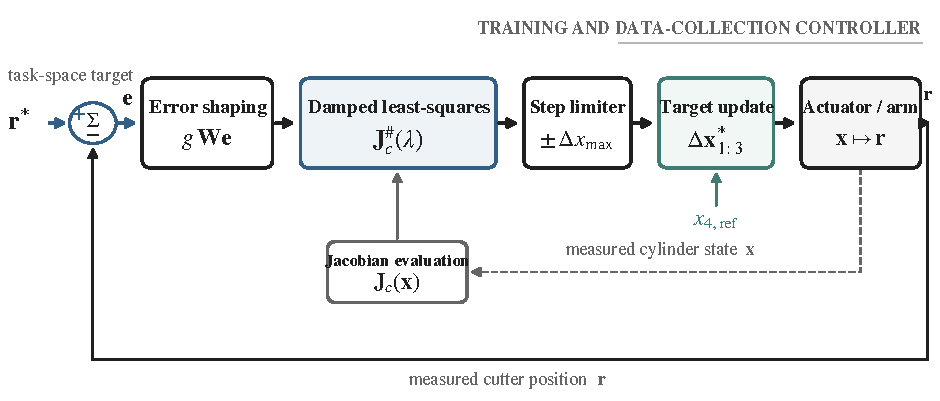
\includegraphics[width=\textwidth]{images/ch6/ch6_dls_controller}
  \caption{Feedback realisation of the damped least-squares teacher of
  \eqref{eq:ctrl:teacher-dls}. The weighted task error is scaled by $g$, mapped
  to the first three cylinder coordinates by the measured damped inverse
  $\bm{J}_c^{\#}(\lambda)$, and clipped to $\pm\Delta x_{\max}$ per tick. Cylinder~4 is
  held at its head-down reference. Cutter position closes the task-space loop
  and the measured cylinder state updates $\bm{J}_c$ at every step. The loop is
  used only for teaching and data collection, never at deployment.}
  \label{fig:ctrl:dls-loop}
\end{figure}


\subsection{Execution Through the Student Interface}

One implementation detail determines whether distillation converges to something
usable. The teacher's output $\Delta\bm{x}^{*}$ is not written to PhysX
directly: it is converted into the same normalised four-value action the student
emits and pushed through the student's entire action chain into the same plant,
so every label the student imitates is by construction an action it can produce.
A teacher writing targets directly to the plant would generate labels outside
the student's reachable set, giving the imitation error a floor no training
could remove.

\subsection{Teacher Performance}

Quoting the teacher's performance is necessary because distillation cannot
exceed it and the gates of Section~\ref{sec:sys:evaluation-criteria} were
anchored to it. Table~\ref{tab:ctrl:teacher} reports the privileged teacher
measured on the stage-6 verge task through the ROM plant, over 128 environments
and 480 control steps.

\begin{table}[tb]
  \centering
  \caption{The privileged DLS teacher, measured on the stage-6 verge task
  through the command-ROM plant (128 environments, 480 steps, all eleven path
  families, seed 17). It is competent, not perfect,
and several evaluation thresholds sit deliberately just outside what it achieves.}
  \label{tab:ctrl:teacher}
  \small
  \begin{tabular}{lcc}
    \toprule
    Quantity & Teacher & Gate \\
    \midrule
    Mean $|e_{\mathrm{cut}}|$        & $\unit[0.0234]{m}$ & $\leq \unit[0.040]{m}$ \\
    p95 $|e_{\mathrm{cut}}|$         & $\unit[0.1524]{m}$ & --- \\
    Mean $|e_{\mathrm{lat}}|$        & $\unit[0.1221]{m}$ & $\leq \unit[0.300]{m}$ \\
    Ground-contact fraction          & $0.7807$ & $\geq 0.700$ \\
    p01 head alignment               & $0.9638$ & $\geq 0.900$ \\
    Minimum head alignment           & $0.8317$ & --- \\
    p95 tool acceleration            & $\unit[64.9]{m/s^2}$ & $\leq \unit[120]{m/s^2}$ \\
    \bottomrule
  \end{tabular}
\end{table}

The teacher is competent but visibly imperfect: it loses ground contact about a
fifth of the time and its cut-height tail is six times its mean. This is why
Section~\ref{sec:sys:evaluation-criteria} re-derived several thresholds, since a
gate set above these numbers could not be passed by the ground-truth controller
itself and would carry no information about the policy.

\section{Policy Formulation}
\label{sec:ctrl:ppo}

\subsection{Policy Definition}

The deployed controller is a memoryless Gaussian multilayer perceptron mapping
a $66$-value observation to four normalised actions. Actor and critic are
separate networks with hidden widths $256$--$128$--$64$, ELU activations and
empirically normalised observations. PPO~\cite{schulman2017proximal} is supplied
by RSL-RL~\cite{rudin2022learning}. This base policy is shared by all three
stacks; \ppoAAMFD{} freezes it and widens the actor input by four plant-context
columns, of which only the payload channel carries information here
(Section~\ref{sec:ctrl:af-residual}).

The four actions denote desired cylinder increments in R and IF and valve
commands in AF (Section~\ref{sec:ctrl:af-fd-sufficient}). The base policy has no
nominal controller beneath it, and the truck's forward motion remains scripted.

\subsection{The Observation Vector}

Figure~\ref{fig:ctrl:observation} lays out the $66$ channels by group. The
grouping tells the story of what this controller has to reason about: nine
terrain-height samples ahead of the cutter, three task-error channels, sixteen
channels of cylinder state and remaining travel, sixteen describing the
actuator interface, ten of pose and context, and twelve of model error.

\begin{figure}[tb]
  \centering
  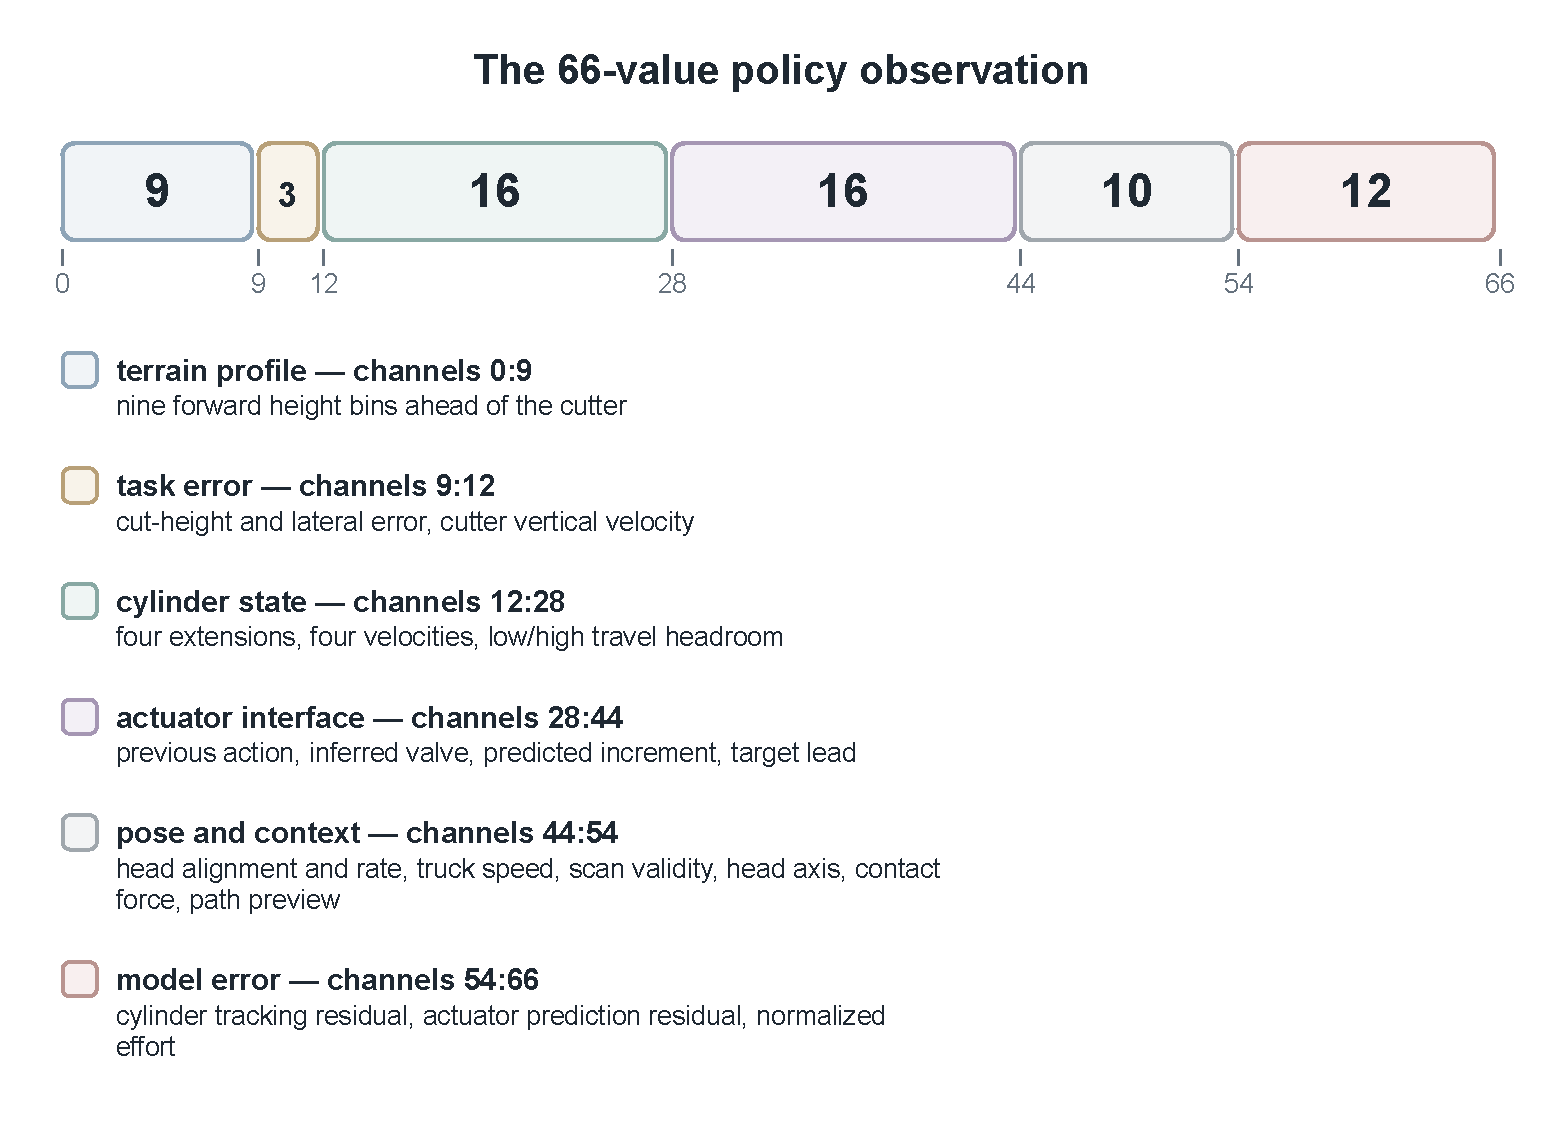
\includegraphics[width=\textwidth]{images/ch6/ch6_observation}
  \caption{The policy observation contract. The six coloured groups form the
  $66$-channel task input shared by R, IF and AF. AF appends the four white
  plant-context inputs in the slice $66{:}70$; only payload varies in the
  reported campaign.}
  \label{fig:ctrl:observation}
\end{figure}

The last twelve channels carry cylinder tracking residual, actuator prediction
residual and normalised effort. A memoryless network cannot form these temporal
errors from one observation, and without them the error to be corrected is
absent from its input. Across ten training blocks, p01 head alignment remained
at $0.79$--$0.80$ when only the feedforward source or levelling gain changed.

This shared contract also limits attribution. The tracking residual is near zero
under R but carries the ID--FD path's standing error under IF, giving IF a useful
closed-loop correction signal. The R--IF comparison therefore cannot separate
the actuator representation from the value of that signal.

\subsection{The Action and Its Bounds}

The policy emits $\bm{a} \in \mathbb{R}^4$, sampled from its Gaussian at
training time and taken at the mean for evaluation. Five bounding stages sit
between that sample and the PhysX cylinder target
(Figure~\ref{fig:ctrl:action-chain}). Each can only reduce authority, never
introduce motion the policy did not request.

\begin{figure}[tb]
  \centering
  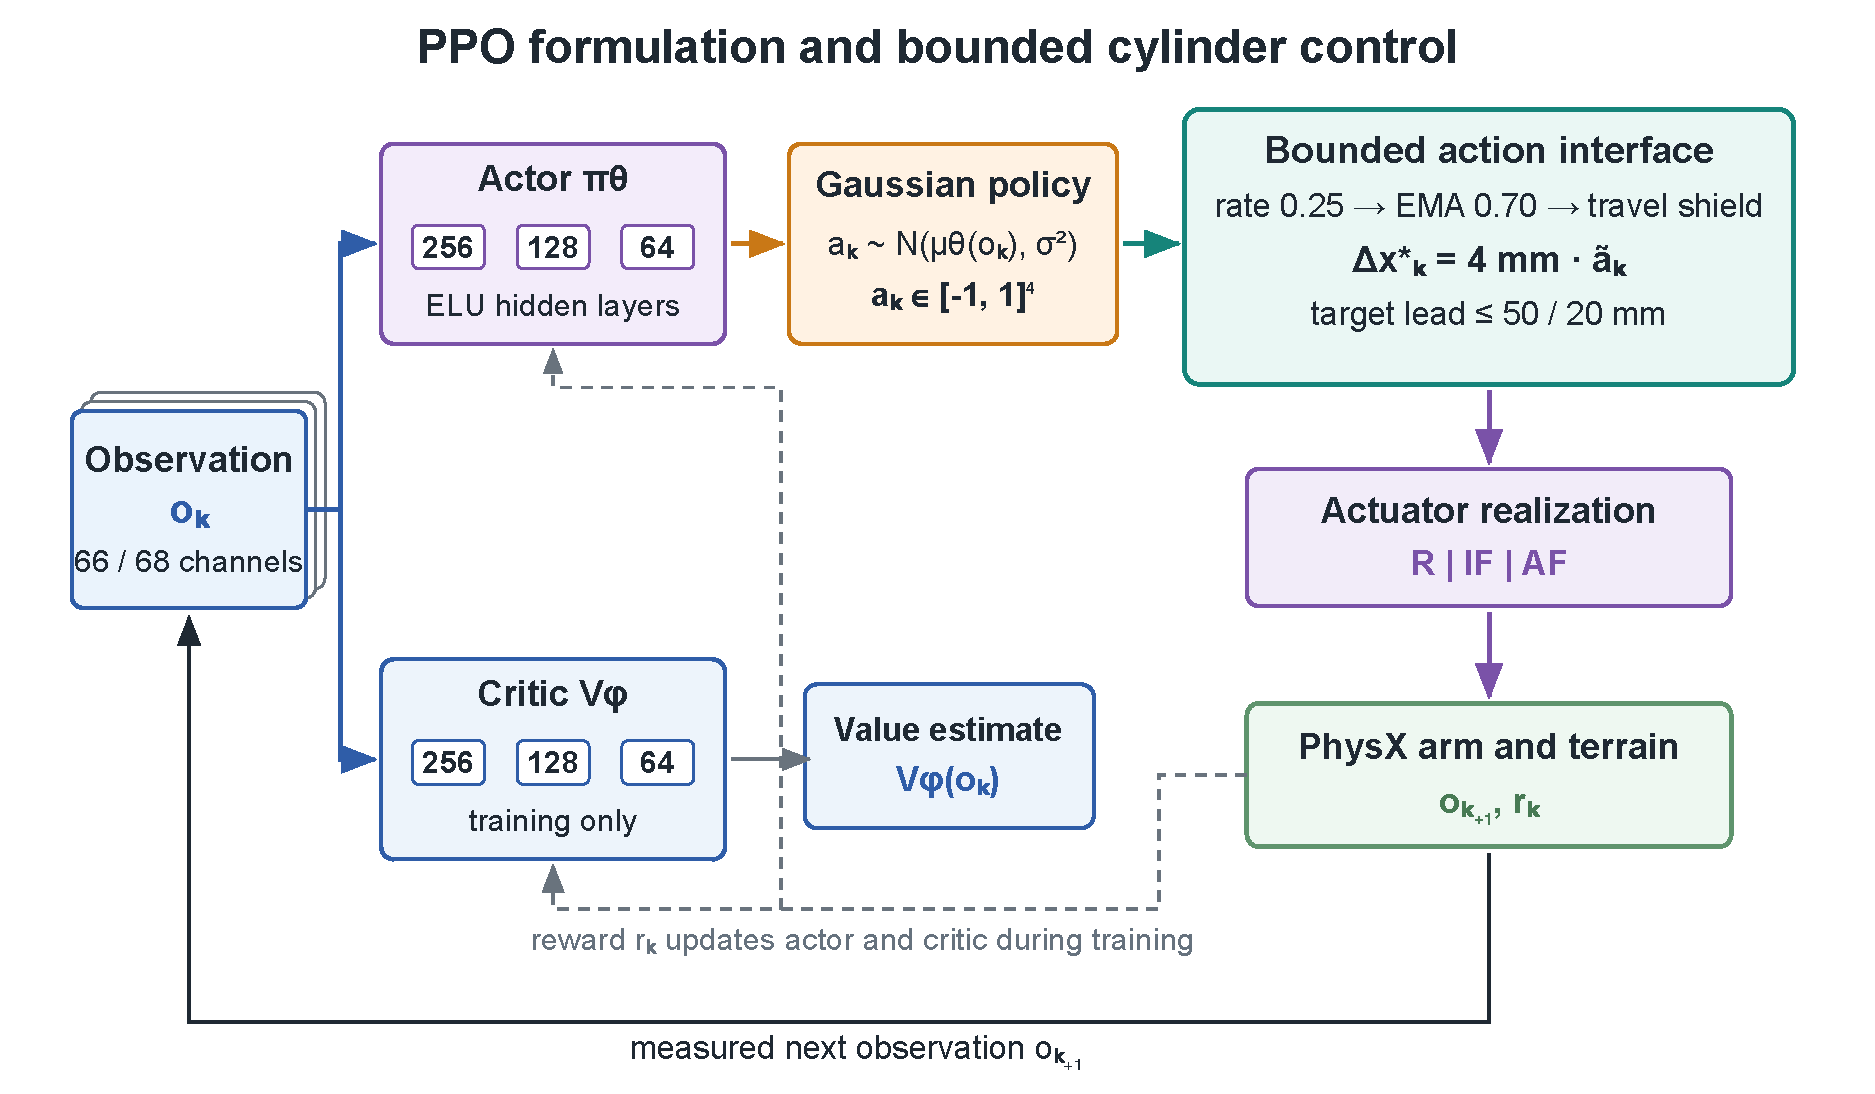
\includegraphics[width=\textwidth]{images/ch6/ch6_action_chain}
  \caption{PPO actor--critic formulation and deployed control path. The actor
  maps the observation to a four-dimensional Gaussian action. Rate limiting,
  exponential filtering, the travel shield, command scaling and the target-lead
  cap bound that action before the selected R, IF or AF actuator path drives
  the PhysX arm. The critic and reward update are training-only; measured state
  closes the deployed loop.}
  \label{fig:ctrl:action-chain}
\end{figure}

The rate limit bounds $|\Delta \bm{a}|$ at $0.25$ per control step and is held
\emph{constant} across every curriculum stage rather than used as a curriculum
knob, by the reachability argument above: the teacher's own command stream has a
structural per-step bound near $0.20$, so a student limit below that makes part
of the label set unreachable. The exponential filter ($\beta = 0.70$ at the
final stage) smooths the command. The limit shield scales the command down, and
only in the direction that consumes headroom, over the last $\unit[20]{mm}$ of
cylinder travel, replacing the teacher's hard clamp into the learned range. The
command scale converts the filtered action into $\unit[4]{mm}$ of cylinder
travel per unit action, and the target integrator accumulates the increments in
reference space, permitted to lead the measured extension by at most
$\unit[50]{mm}$ on cylinders~1 to~3 and $\unit[20]{mm}$ on cylinder~4.

This is the cylinder-increment reading of the action, used by \ppoROM{} and
\ppoIDFD{}. Under \ppoAAMFD{} the same bounded action is a valve command scaled
to span the admissible valve range, so the cylinder-space stages do not carry
the same meaning there.

The lead cap is load-bearing. Raising it to $\unit[50]{mm}$ halved lateral error
on \texttt{lane\_change\_hold} ($0.4833 \to 0.2310$) and
\texttt{boom\_sweep} ($0.3745 \to 0.1602$), but applying the same value to
cylinder~4 reduced head alignment from $0.9507$ to $0.4636$. This measured split
sets the per-axis limits above.

The chain also fixes the capability ceiling: four millimetres of cylinder travel
per step is the entire authority budget, which produces the
$\unit[0.240]{m/s}$ lateral rate limit of Section~\ref{sec:sys:capability} from
which the reference paths are derived.

\subsection{The Reward Function}

The final \ppoROM{} reward has ten bounded terms
(Table~\ref{tab:ctrl:reward}): three task rewards and seven behaviour penalties.
All retain a gradient beyond the acceptance boundary. Three rules govern them,
each adopted after a measured failure.

\paragraph{No Gaussian Shaping}
The earlier reward priced tracking as $w\exp[-(e/s)^2]$, which is effectively
flat beyond about $2s$ and therefore supplies almost no gradient where the
failing path families live. Every shaping term is instead linear or Huber in the
error. Writing $x = |e|/s$, the two shapes used are
%
\begin{equation}
  \label{eq:ctrl:shapes}
  B(e;s,c) = \min(x,\,c),
  \qquad
  H(e;s,c) = \min\Bigl(c,\;
  \begin{cases}
    \tfrac{1}{2}x^{2}, & x \le 1\\
    x - \tfrac{1}{2},  & x > 1
  \end{cases}\Bigr).
\end{equation}
%
$B$ has the same gradient at $\unit[0.5]{m}$ of error as at $\unit[0.05]{m}$,
so a policy far from the reference is still told which way to move; $H$ buys
quadratic precision near zero where cut height needs it, without a vanishing
far field.

\paragraph{Bounded Terms}
An unbounded term can dominate the sum and destabilise the critic. Each
contribution is clipped, giving the reward a published budget: $6+12+4 = 22$ for
the task terms against $-24$ for the safety terms. A non-finite value is
replaced by $-25$, just below that worst case, so a numerical fault can never
outscore legitimate behaviour.

\paragraph{Fixed Sign Convention}
The three task terms are non-negative and the seven safety terms non-positive.
This makes worst-case (CVaR) weighting~\cite{rockafellar2000cvar} safe: scaling
a non-positive term by a factor $\ge 1$ can only lower return. Earlier positive
worst-case weights instead rewarded poor environments, while an action-magnitude
penalty discouraged the sustained offsets required by three path families.

\begin{table}[tb]
  \centering
  \caption{The ten reward terms of the final \ppoROM{} task, with weights and
  shaping scales. $B$ and $H$ are the bounded shapes of
  Equation~\eqref{eq:ctrl:shapes}. The lateral and head terms each combine a
  coarse and a fine scale, so far-field correction and near-field precision are
  priced separately.}
  \label{tab:ctrl:reward}
  \small
  \begin{tabular}{llp{6.0cm}}
    \toprule
    Term & Weight & Shape and purpose \\
    \midrule
    Cut-height tracking & $+6$   & $H$, scale $\unit[0.04]{m}$, cap $2.5$; the
      primary mowing-quality term \\
    Lateral tracking    & $+12$  & $B$, coarse $\unit[1.50]{m}$ and fine
      $\unit[0.60]{m}$ mixed $0.6/0.4$; the primary line-following term \\
    Ground contact      & $+4$   & pays for the cutter being in contact \\
    Head alignment      & $-12$  & $B$ on the deficit below $0.98$, fine scale
      $0.02$ and coarse scale $1.00$ mixed evenly \\
    Contact loss        & $-3$   & charges directly for loss of contact \\
    Action rate         & $-1$   & $B$ on the mean absolute command change,
      scale $0.25$; penalizes chatter \\
    Tool acceleration   & $-1$   & $B$, scale $\unit[300]{m/s^2}$;
      mechanical-wear proxy on the cutter \\
    Contact force       & $-1$   & $B$ on force above $\unit[30]{kN}$, scale
      $\unit[150]{kN}$ \\
    Cylinder headroom   & $-2$   & $B$ on encroachment inside a
      $\unit[0.02]{m}$ margin, scale $\unit[0.10]{m}$ \\
    Hard impact         & $-4$   & indicator on the impact event \\
    \bottomrule
  \end{tabular}
\end{table}

One apparent inconsistency is deliberate. The tool-acceleration term saturates
at $\unit[300]{m/s^2}$ while its gate sits at $\unit[120]{m/s^2}$, because the
reward scale is a saturation scale for a bounded penalty rather than a target:
the gate stays the binding criterion and the reward only keeps a gradient
against gross excursions. The action-rate term is mild for a related reason,
since cylinder~4 owns head pitch and a rate tax falls hardest on the fast
corrections that keep the head down.

Every term is logged by name during training, because total reward can rise
while the system gets worse. The reward is not the result criterion; promotion
uses the eight gates of Section~\ref{sec:sys:evaluation-criteria}.

\subsection{Optimisation}
\label{sec:ctrl:optimization}

Policies are optimised with clipped-surrogate PPO over generalised advantage
estimation, in the form of Section~\ref{sec:fund:rl-residual}. The maintained
configuration uses clip parameter $\epsilon = 0.2$, discount $\gamma = 0.99$,
GAE parameter $\lambda = 0.95$, five learning epochs over four minibatches per
update, an adaptive learning-rate schedule targeting a KL divergence of $0.02$
from a base rate of $3\times10^{-4}$, gradient-norm clipping at $1.0$, and a
clipped value loss with coefficient $1.0$. The terrain task collects $32$ steps
per environment per update. At $512$ environments that is $16\,384$ transitions
per update, chosen because the inherited $128$-step horizon exceeded two
minutes per update on the available GPU without adding useful batch diversity.

The final fine-tuning blocks depart from that configuration because they run
under the reference anchor of Section~\ref{sec:ctrl:anchored} rather than an
adaptive learning-rate schedule: clip $\epsilon = 0.1$, discount
$\gamma = 0.97$, three learning epochs, fixed learning rates of $10^{-5}$ for
the actor and $10^{-4}$ for the critic, entropy coefficient $0.001$, an
exploration standard deviation fixed at $0.15$ and excluded from the gradient,
and frozen observation normalisers.

These departures reflect the locally controlled task and the anchor. The shorter
discount credits actions for the terrain state they face, the actor changes more
slowly than the critic, and the fixed learning rate avoids competing with the
explicit divergence bound. Because zero action leaves the arm stationary, early
training used a standard deviation of $0.30$ to discover command directions.
Distilled terrain policies instead use the smaller fixed value above. Exact run
values remain recorded in each frozen manifest.

\section{Training Protocol and the Distillation Finding}
\label{sec:ctrl:training}

\subsection{Distillation by DAgger}

Policies are initialised by imitation, not by reward. The privileged teacher is
rolled out in the student's own environment and the student is fitted to the
teacher's raw action by regression, in the DAgger scheme of Ross et
al.~\cite{ross2011reduction}: the teacher's probability of \emph{executing} the
action, rather than merely labelling it, is annealed from one to zero over the
first $70\,\%$ of iterations, so later training collects states the student
itself visits. Labels are accumulated in a replay buffer of $262\,144$
transitions and refitted over three epochs per iteration in minibatches of
$8\,192$.

Figure~\ref{fig:ctrl:distillation} shows a complete distillation run for the
ROM stack, taken from the stored record. The behaviour-cloning loss falls by
more than an order of magnitude while the teacher is still driving, reaches its
minimum around the handover, and then \emph{rises} once the student is alone.
That rise is the distribution shift DAgger exists to expose rather than a
failure: the student is now visiting states the teacher never chose, and the
teacher's advice on those states is new information. The closed-loop task
metrics remain near the teacher's preflight values without matching them.

\subsection{Objective Mismatch in Unconstrained Fine-Tuning}
\label{sec:ctrl:finding}

Unconstrained PPO fine-tuning from distilled checkpoints increased total reward
while degrading the primary tracking objective, in the worst case by a factor
of $12.9$. The critic remained healthy, with explained variance in the
$0.85$--$0.95$ range. This motivates the anchored formulation of
Section~\ref{sec:ctrl:anchored}, which is used for the final policies.

The reward includes ground contact and cut height as well as lateral tracking,
so it can increase while a gate-relevant tracking measure degrades. This is a
claim about two functionals over the same policy space rather than about the
optimiser. Training maximizes the expected return
$J(\vartheta)$, while acceptance is decided by the vector of physical gates
$\bm{G}(\vartheta) \preceq \bm{g}^{\star}$ of
Section~\ref{sec:sys:evaluation-criteria}. Writing
$\mathcal{F} = \{\vartheta : \bm{G}(\vartheta) \preceq \bm{g}^{\star}\}$ for the
feasible set, the measured content of the finding is
%
\begin{equation}
  \label{eq:ctrl:mismatch}
  \arg\max_{\vartheta} J(\vartheta) \notin \mathcal{F},
  \qquad\text{while}\qquad
  \vartheta_{\mathrm{distilled}} \in \mathcal{F}.
\end{equation}
%
The teacher places the distilled policy inside $\mathcal{F}$, whereas
unconstrained ascent optimises a different functional and may leave it. The
protocol therefore reports both checkpoints, logs gate metrics during training
and constrains policy drift from the point where reward and evaluation were
known to agree.

\section{Reference-Anchored PPO}
\label{sec:ctrl:anchored}

Equation~\eqref{eq:ctrl:mismatch} says that reward ascent leaves the feasible
set. It does not say that reward ascent is useless, only that it is unbounded.
The construction of this section keeps PPO and constrains how far it may travel
from a policy already known to satisfy the gates. Writing $\pi_{\mathrm{ref}}$
for a frozen reference policy and $J$ for the expected return, each training
block solves
%
\begin{equation}
  \label{eq:ctrl:constrained}
  \max_{\vartheta} J(\vartheta)
  \quad \text{s.t.} \quad
  \mathbb{E}_{\bm{o}\sim d_{\pi_\vartheta}}
  \bigl[ \mathrm{KL}\bigl( \pi_{\mathrm{ref}}(\cdot\,|\,\bm{o})
  \,\|\, \pi_\vartheta(\cdot\,|\,\bm{o}) \bigr) \bigr]
  \le \delta_{\mathrm{ref}},
\end{equation}
%
with the expectation taken over the states the policy itself visits.

\subsection{Critic Warm-Up}

After distillation the actor already behaves sensibly, but the critic has never
been fitted to the long terrain return, so the first PPO updates would move a
useful actor using a value estimate that is not yet meaningful. The actor is
frozen for $150$ iterations while only the value loss is optimised, under the
asserted invariant $\vartheta_{\text{after}} = \vartheta_{\text{before}}$. The
observation normalisers are frozen at the same point, since otherwise the same
raw observation is normalised differently from one iteration to the next and the
actor's behaviour changes while its weights do not.

\subsection{The Reference Anchor}

Let $\pi_{\mathrm{ref}}$ be a frozen copy of the accepted warm actor. It is
queried only on states the live policy visits and never supplies an executed
action, so PPO remains the sole controller of the plant. The penalty is the
\emph{forward} divergence, which for diagonal Gaussians is available in closed
form~\cite{cover2006information},
%
\begin{equation}
  \label{eq:ctrl:kl}
  D_{\mathrm{ref}}
  = \mathrm{KL}\bigl(\pi_{\mathrm{ref}} \,\|\, \pi_\vartheta\bigr)
  = \sum_i \left[
    \log\frac{\sigma_{\vartheta,i}}{\sigma_{\mathrm{ref},i}}
    + \frac{\sigma_{\mathrm{ref},i}^{2}
      + (\mu_{\mathrm{ref},i}-\mu_{\vartheta,i})^{2}}
      {2\sigma_{\vartheta,i}^{2}}
    - \frac{1}{2}\right],
\end{equation}
%
at the cost of one additional forward pass and no sampling. Because both scales
are fixed at $\sigma = 0.15$, this collapses to a pure quadratic on the drift of
the commanded action,
%
\begin{equation}
  \label{eq:ctrl:kl-fixed}
  D_{\mathrm{ref}}
  = \sum_i \frac{(\mu_{\mathrm{ref},i}-\mu_{\vartheta,i})^{2}}{2(0.15)^{2}},
\end{equation}
%
which is the second reason for fixing $\sigma$: with a free standard deviation,
entropy collapse shrinks $D_{\mathrm{ref}}$ while the commanded action moves, so
the constraint would report compliance during the drift it exists to prevent.

Forward KL penalises abandoning any reference behaviour; reverse KL could
collapse onto a subset, reproducing the observed trade between competencies.
The term is therefore a behaviour-cloning anchor on the live policy's states,
following demonstration-regularised policy gradient~\cite{rajeswaran2018dapg}.

The actor objective is
%
\begin{equation}
  \label{eq:ctrl:anchored-loss}
  \mathcal{L}(\vartheta)
  = \mathcal{L}_{\mathrm{PPO}}
  + \mathcal{L}_{V}
  - \beta\,\mathcal{H}(\pi_\vartheta)
  + \lambda_{\mathrm{ref}}\,
    \mathbb{E}_k\bigl[\mathrm{KL}(\pi_{\mathrm{ref}} \| \pi_\vartheta)\bigr],
  \qquad
  \lambda_{\mathrm{ref}} = 0.10 .
\end{equation}

\subsection{Trust Regions and Rollback}

A penalty is not a constraint: at a fixed coefficient, a sufficiently large
advantage always buys its way past. Feasibility is therefore also verified on the update taken. Two bounds are imposed,
%
\begin{equation}
  \label{eq:ctrl:bounds}
  D_{\mathrm{update}} = \mathrm{KL}(\pi_{\mathrm{old}} \| \pi_\vartheta)
  \le 0.01,
  \qquad
  D_{\mathrm{ref}} \le 0.05,
\end{equation}
%
and they do different work. $D_{\mathrm{update}}$ is the classical step-size
control that keeps the surrogate a valid local model of $J$.
$D_{\mathrm{ref}}$ is the new object: because the anchor is \emph{fixed} within
a block rather than moving with the policy, it bounds cumulative drift. A
sequence of updates each individually satisfying $D_{\mathrm{update}}$ can
still walk arbitrarily far from feasibility, and that is the trajectory the earlier campaigns took, monotonically, with the reward rising the whole
way. Only a constraint referred to a fixed feasible point can observe it.

Enforcement is in two stages. During minibatch optimisation the epoch is
early-stopped as soon as $D_{\mathrm{update}}$ exceeds its bound, and after the
update both divergences are recomputed over the full rollout. If either bound
fails, or any quantity is non-finite, the actor and its optimiser state are
restored \emph{atomically}. On a divergence rejection the critic fit is retained
when finite, since the bounds constrain the policy rather than the value
function; on a non-finite update both networks are restored. In the final block,
five of one hundred logged updates were rejected, all on the reference bound and
none on the update bound, so the drift caught was of the kind ordinary PPO
clipping does not see.

\subsection{The Block Ratchet}

The reference is not fixed forever. Within a block it is frozen. When a
checkpoint is scored and passes the gates, it is promoted to reference,
%
\begin{equation}
  \label{eq:ctrl:ratchet}
  \vartheta_{\mathrm{ref}}^{(m+1)} = \vartheta^{\star},
  \qquad
  \vartheta^{\star} \in \mathcal{F},
  \quad
  \vartheta^{\star} \in
  B_{\delta_{\mathrm{ref}}}\bigl(\vartheta_{\mathrm{ref}}^{(m)}\bigr),
\end{equation}
%
and the actor's optimiser moments are reset, because momentum accumulated
relative to the old anchor is not meaningful relative to the new one. The
critic's are retained: it is fitting the same return, and its calibration is
expensive to rebuild.

The anchor advances only through checkpoints verified against $\bm{G}$, bringing
the evaluation criterion into training. Distillation supplies the first anchor;
the critic is warmed with actor and normalisers frozen; each later block trains
within the fixed bound, rolls back rejected updates, scores checkpoints on at
least three held-out meshes and promotes only a passing checkpoint. The last
promotion is returned. Algorithm~\ref{alg:ctrl:anchored} in
Appendix~\ref{app:anchored-ppo} gives the full procedure.



\subsection{Theoretical Status}
\label{sec:ctrl:theory}

The components are standard and citable. The bound on $D_{\mathrm{update}}$ is
conservative policy iteration and its trust-region
descendants~\cite{kakade2002approximately,schulman2015trust}; the atomic
rollback is that literature's backtracking line search reduced to a single
trial point; the penalty in Equation~\eqref{eq:ctrl:anchored-loss} is a
Lagrangian relaxation of the constrained problem~\eqref{eq:ctrl:constrained} at
a fixed multiplier, with the rollback supplying the feasibility enforcement a
fixed multiplier cannot.

What does not follow is a certificate. Bounding the divergence from a verified
policy does bound gate degradation in form, since the chain rule of KL over
trajectories, Pinsker's inequality and the boundedness of every gate metric give
$|\mathbb{E}_{\pi_\vartheta}[g] - \mathbb{E}_{\pi_{\mathrm{ref}}}[g]|
\le 2 G_{\max}\sqrt{H \delta_{\mathrm{ref}}/2}$ for a metric $g$ with
$\|g\|_\infty \le G_{\max}$ over a horizon $H$
(Appendix~\ref{app:kl-bound} derives this bound step by step). At the
production horizon of $2808$ steps and $\delta_{\mathrm{ref}} = 0.05$ the
right-hand side exceeds sixteen, which for a metric bounded in $[0,1]$ is
vacuous, and there is a further measure mismatch because the constraint is
taken under the live policy's state distribution while the chain rule requires
the reference's. The construction is therefore a principled restriction of
reward ascent to a neighbourhood of a verified policy, not a guarantee: the
gates certify each promotion.

\section{R: Reference Actuator Baseline}
\label{sec:ctrl:ppo-rom}

\ppoROM{} is the reference condition. The policy emits desired cylinder motion,
the frozen command ROM converts it to a cylinder target, and PhysX closes the
loop. The scripted truck crosses a $\unit[26]{m}$ strip at a constant speed
drawn per episode from $2$ to $\unit[7]{km/h}$; path families and terrain meshes
are distributed across environments.

It is a reference condition rather than a competitor: ROM-plus-PhysX \emph{is}
the deployment plant, so \ppoROM{}'s actuator coincides with the plant. What
that does to its tracking advantage is stated in
Section~\ref{sec:ctrl:matching}.

The policy follows the chapter's three-stage construction: distillation, frozen
actor critic warm-up and reference-anchored PPO. Checkpoints $280$--$329$ were
scored on held-out meshes against the eight gates, with worst-mesh and, where
applicable, worst-family aggregation. Chapter~\ref{chap:evaluation} reports the
common-protocol evaluation.

\section{IF: Non-Adaptive Learned Baseline}
\label{sec:ctrl:ppo-idfd}

\ppoIDFD{} subclasses the \ppoROM{} task and changes exactly one thing. The
policy still emits desired cylinder motion, but that command is now realised by
the frozen inverse model of Section~\ref{sec:models:id}, which converts it to a
valve command, followed by the frozen strict forward model of
Section~\ref{sec:models:fd}, which converts the valve command to a predicted
extension increment. PhysX receives the same bounded cylinder target as before.
Task, terrain families, meshes, observation contract, action chain, reward,
gates and the PPO update are inherited unchanged, so the actuator
representation is the only free variable between the two stacks.

\emph{Robust} here means what Section~\ref{sec:fund:domain-randomization} means
by it: trained across the randomised plant family, applying one fixed response
to whichever member it meets, with no online estimation. The policy is not blind
to plant variation, since the twelve model-error channels carry a standing
residual that is itself plant-dependent. What it lacks is any representation of
\emph{which} plant produced them.

Two properties of the composed path shape its behaviour, both established
offline. The valve command is accumulated rather than issued absolutely and is
clipped to the per-axis limits $[0.95, 0.95, 0.80, 0.80]$, so the actuator path
carries its own saturation boundary independently of the action chain. Only the
predicted extension increment is integrated; the velocity output is a
diagnostic (Section~\ref{sec:models:fd}).

The stored run manifest matches \ppoROM{} field for field on actor learning
rate, entropy coefficient, seed, terrain seed, environment count, curriculum
stage, frozen normaliser and warm-up, which is what makes the pair a controlled
comparison.

\begin{figure}[!htbp]
  \centering
  \makebox[\textwidth][c]{%
    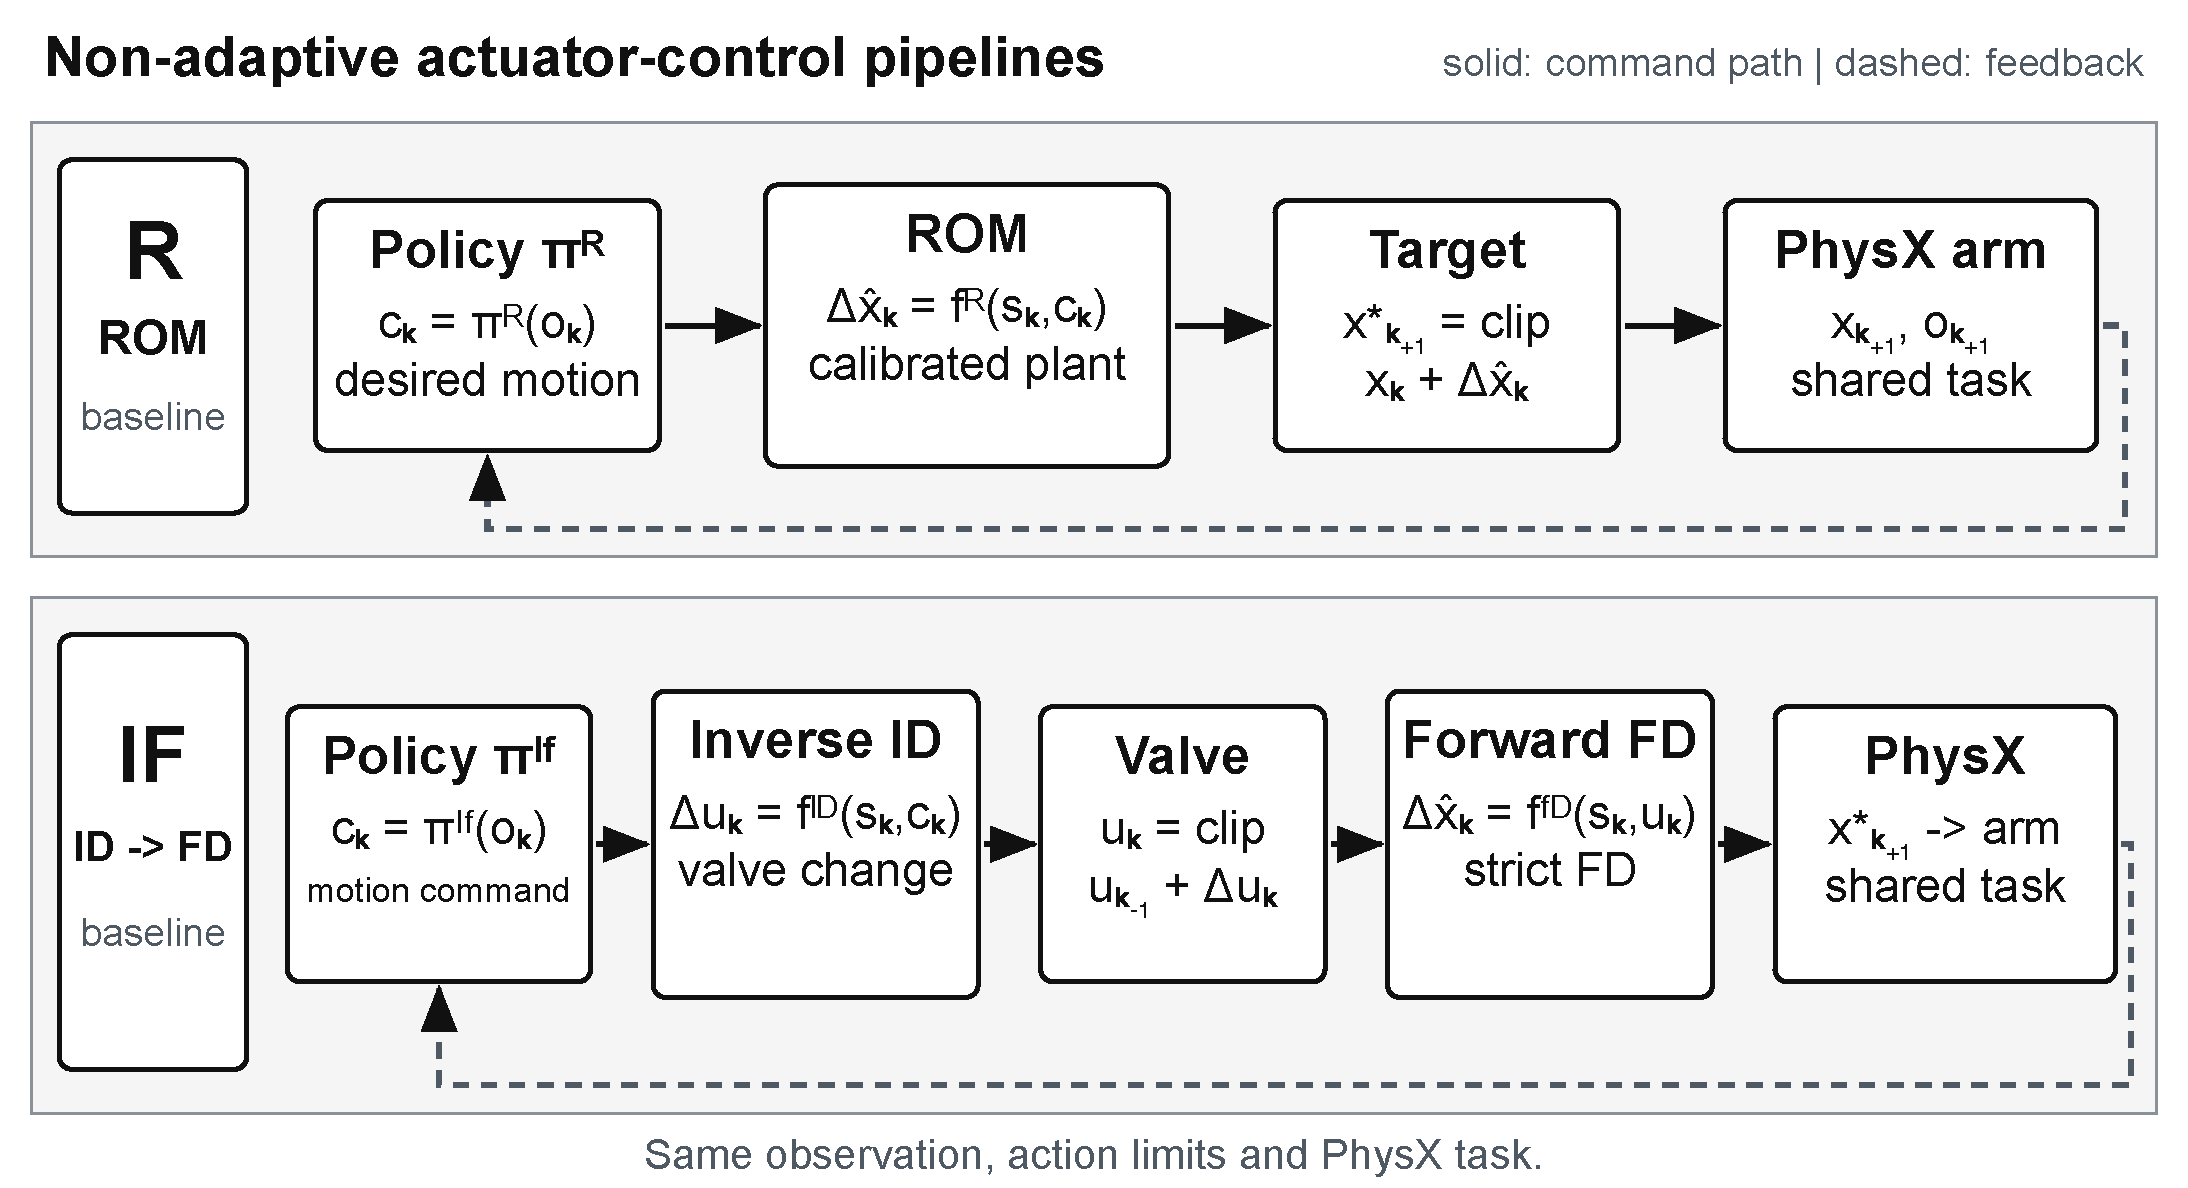
\includegraphics[width=1.08\textwidth]{images/ch6/ch6_r_if_stack}}
  \caption{The non-adaptive R and IF control pipelines. R sends the policy's
  desired cylinder motion through the calibrated command ROM. IF composes the
  independently identified inverse and strict forward models before applying
  the same bounded cylinder target in PhysX. Both paths use the same
  observation, action limits and task.}
\label{fig:ctrl:r-if-stack}
\end{figure}

\section{AF: The Adaptive Stack}
\label{sec:ctrl:ppo-aamfd}

Table~\ref{tab:ctrl:af-matching} states what AF shares with R and IF and what it
does not. AF is not a matched replacement for IF: it answers whether conditioning on an
online payload estimate can improve a frozen direct-valve controller once the
saturated inverse-model command path has been removed. The matched
actuator-representation comparison remains R against IF, and adaptation is
evaluated inside AF against its own frozen and wrong-information controls. This
is stated once here and not repeated.

\begin{table}[H]
  \centering
  \caption{What is matched between AF and the R/IF pair, and what is not.
  Section~\ref{sec:ctrl:matching} gives the full matching rules.}
  \label{tab:ctrl:af-matching}
  \small
  \begin{tabular}{@{}l c p{0.46\textwidth}@{}}
    \toprule
    Dimension & Matched? & Detail \\
    \midrule
    Task, terrain, reward, gates & yes & identical across all three stacks \\
    Base $66$-channel observation & yes & AF appends four context columns
      derived from these channels \\
    Action contract & no & AF emits the valve command directly, not a
      bounded cylinder increment \\
    Training seed & no & AF trains at a different seed \\
    Actor learning rate & no & lower than the R/IF value \\
    Frozen-actor warm-up & no & AF's base is the already-distilled policy,
      frozen; there is no separate warm-up stage \\
    \bottomrule
  \end{tabular}
\end{table}

\ppoAAMFD{} places online adaptation on the forward model alone. The policy
emits the valve command directly, the frozen strict forward model of
Section~\ref{sec:models:fd} converts that command to a predicted extension
increment, and PhysX receives the same bounded cylinder target as the other two
stacks:
%
\begin{equation}
  \label{eq:ctrl:af-path}
  \pi_{\mathrm{frozen}}(\bm{o},\, \hat{\bm{c}})
  \;\longrightarrow\; \bm{u}
  \;\longrightarrow\; f_{\mathrm{FD}}
  \;\longrightarrow\; \text{PhysX} .
\end{equation}
%
The inverse model is absent from the command path. The final AF stack is the
frozen direct-valve base actor, four trained context columns carrying the
estimate $\hat{\bm{c}}$, and the frozen strict forward model; the offline AAM of
Chapter~\ref{chap:models} is not part of it. Zeroing the estimate exactly
recovers the frozen base, and permuting it across environments preserves its
distribution while destroying its pairing, which are the controlled comparisons
used in Chapter~\ref{chap:evaluation}.

Instrumentation confirms that the direct-valve path applies neither inverse-model
valve elements nor adapters at that site. The checkpoint key
\texttt{id\_aam\_fd} is retained only for compatibility with earlier runs.

\begin{figure}[!htbp]
  \centering
  \makebox[\textwidth][c]{%
    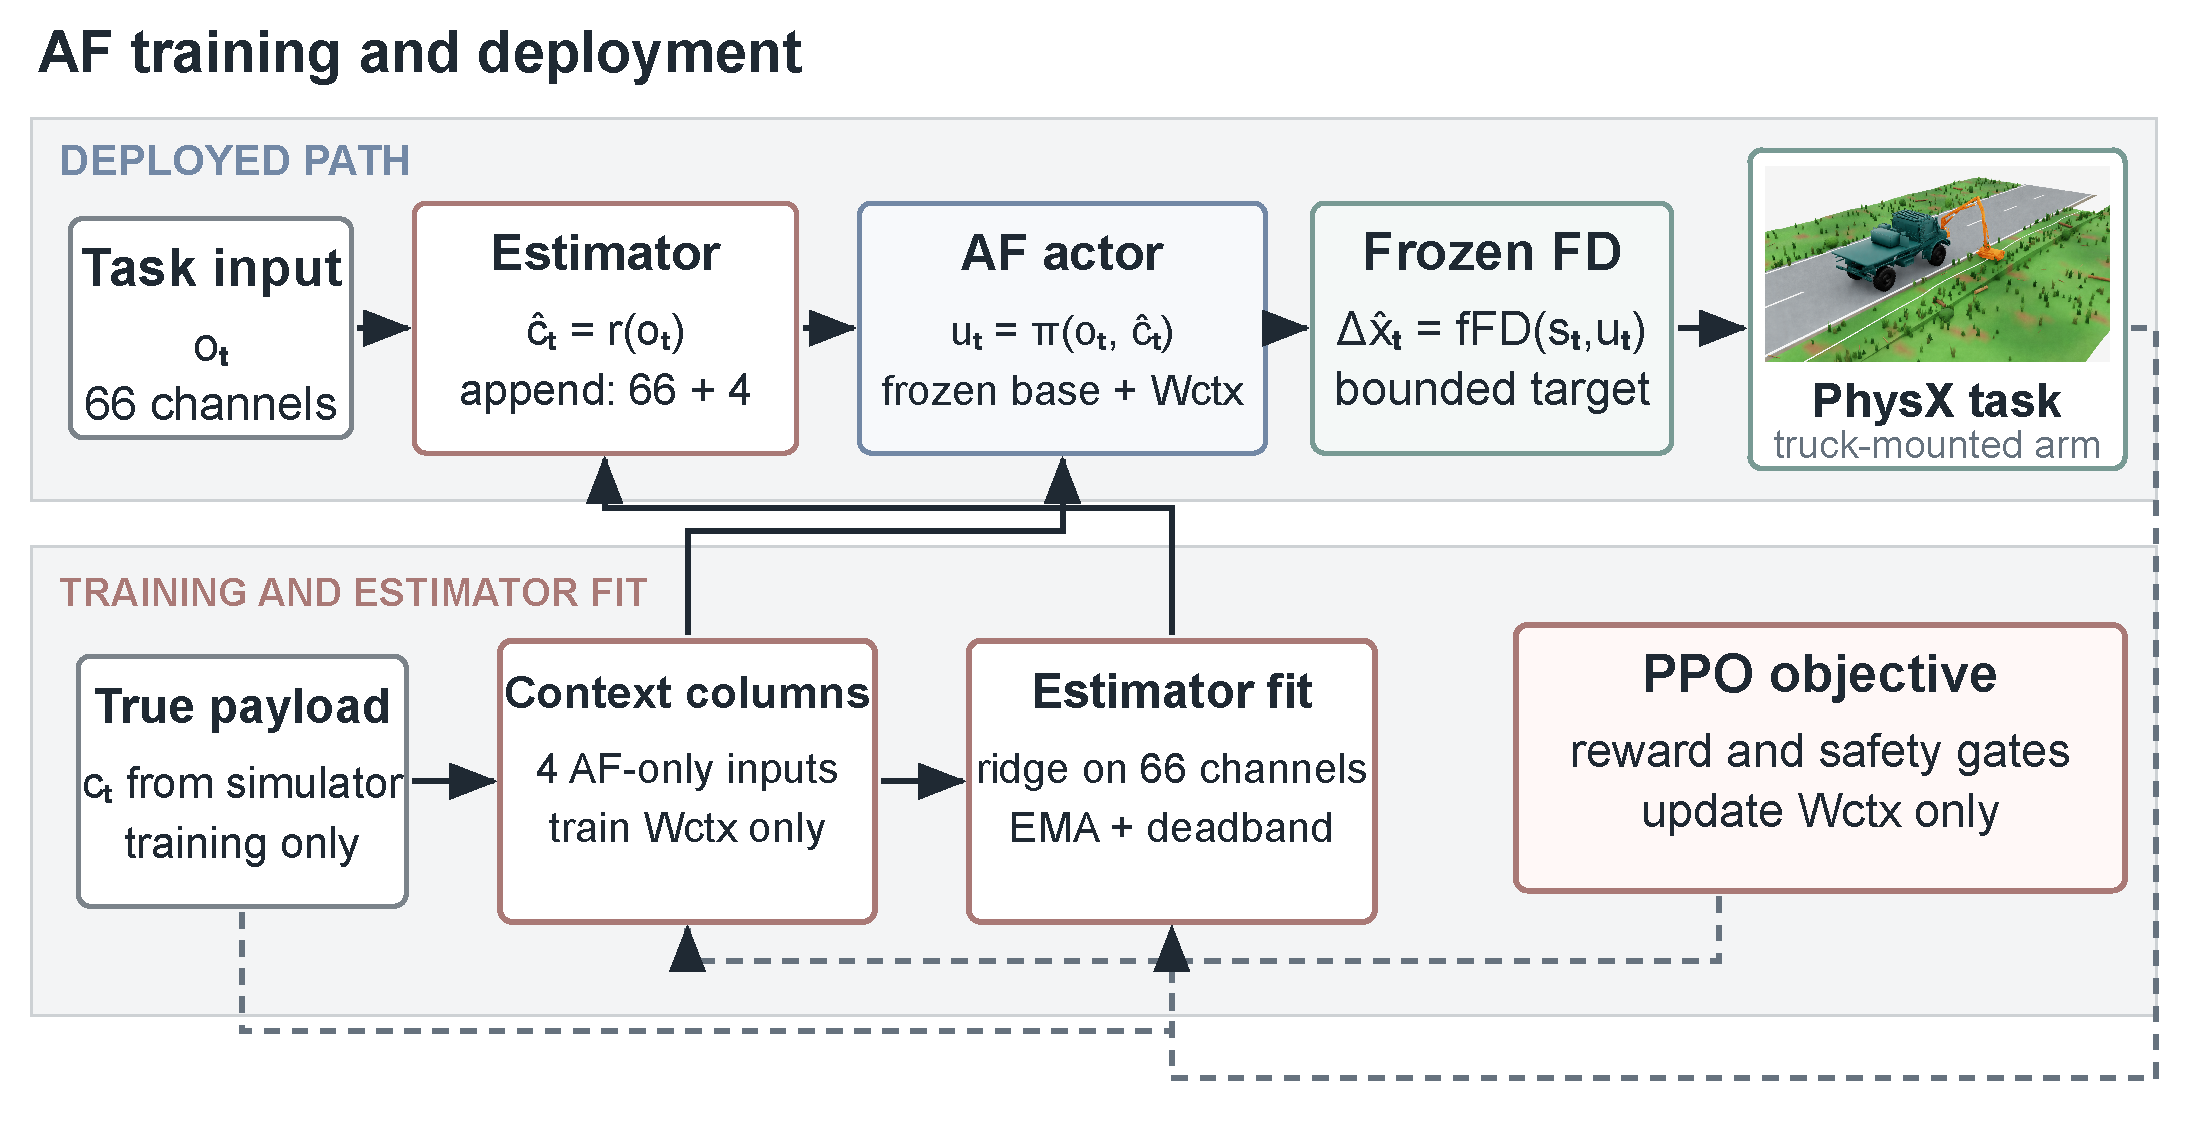
\includegraphics[width=1.08\textwidth]{images/ch6/ch6_aam_stack}}
  \caption{AF training and deployment. A ridge estimator maps the $66$-channel
  task input to four AF-only context values, applies EMA and a deadband, and
  appends them to the actor input. The actor combines its frozen base with
  $\bm{W}_{\mathrm{ctx}}$ and sends valve commands through Frozen FD to PhysX.
  During training, true payload supplies the context inputs and PPO updates only
  the $1\,024$ weights of $\bm{W}_{\mathrm{ctx}}$; the estimator is fitted
  afterwards on trained-policy rollouts. Dashed paths show updates and fitting
  data.}
\label{fig:ctrl:aam-stack}
\end{figure}

\begin{figure}[!htbp]
  \centering
  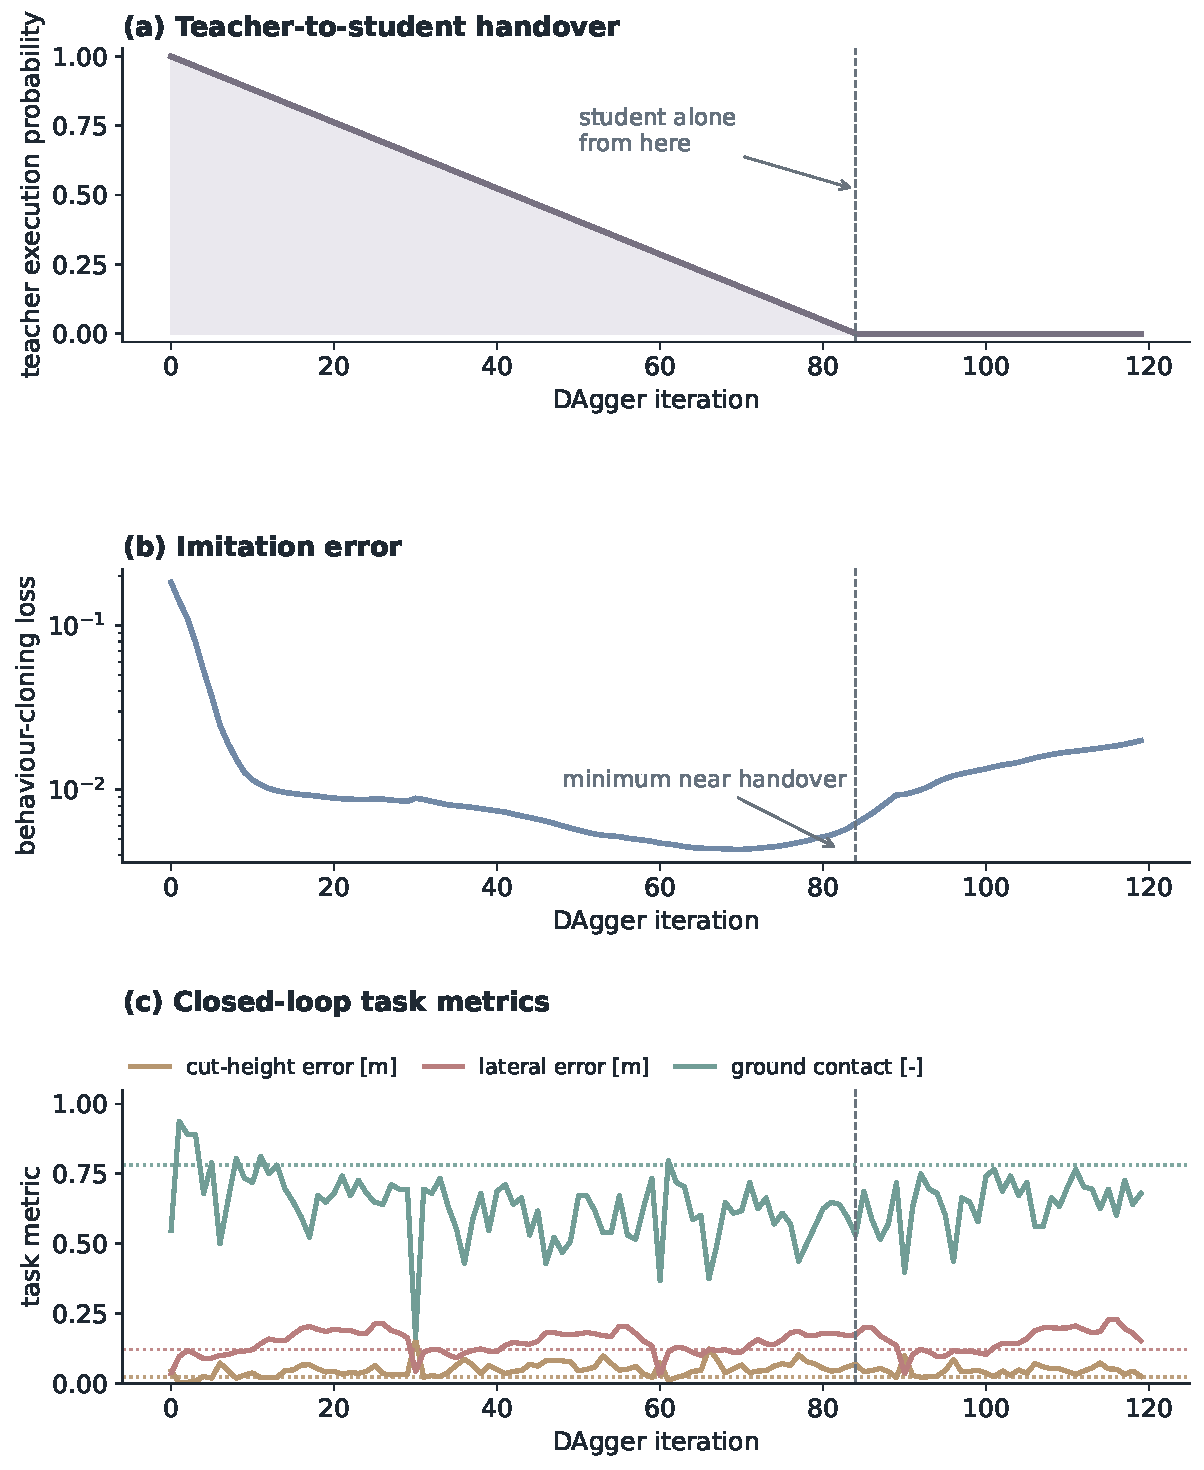
\includegraphics[width=\textwidth]{images/ch6/ch6_distillation}
  \caption{A measured distillation run for the \ppoROM{} stack. (a)~The
  teacher's execution probability falls to zero over the first $70\,\%$ of
  iterations. (b)~Behaviour-cloning loss falls by over an order of magnitude
  under teacher execution, then rises as the student visits new states.
  (c)~Cut-height error, lateral error and ground-contact fraction; dotted lines
  mark the teacher's preflight values from Table~\ref{tab:ctrl:teacher}.}
  \label{fig:ctrl:distillation}
\end{figure}


\subsection{Omission of the Inverse Model}
\label{sec:ctrl:af-no-id}

The inverse model belongs in \ppoIDFD{} and not in the adaptive stack, and the
reason is the same measurement in both cases. \ppoIDFD{} prices the cost of
substituting an independently identified pair for the deployment plant, and that
question needs the inverse model: a policy commanding desired cylinder motion
needs a map from intent to valve command, and supplying that map from
identification data alone is the substitution being priced.

Adaptation needs something the same map cannot give. Because the model predicts
a valve-command \emph{increment} that is accumulated and clipped
(Section~\ref{sec:models:id}), sustained demand walks the command onto its limit
and holds it there. Fed its own predictions the composite left the reference in
every one of the $118$ runs, with the pre-clip command at its limit on
$89.1\,\%$ of elements while the ROM valve on the same runs never reached its
bound. Closed-loop instrumentation over the $33$-cell panel says the same thing
in adaptation's terms: the command sat at its pre-clip limit on $79.9\,\%$ of
valve elements, $34.5\,\%$ of computed corrections were clipped away, and on
$37.9\,\%$ of elements the correction could not move the command at all.

The quantity being adapted and the quantity being saturated are therefore the
same, which makes a null through that path uninterpretable: it cannot separate a
task that is not adaptation-limited from credit clipped before it reached the
metric. Nothing here retracts what is claimed for \ppoIDFD{}, where the command
is consumed as issued. The final stack emits the valve command directly, so the
conditioning acts on the same bounded command as the policy.

\subsection{Sufficiency of the Forward Model}
\label{sec:ctrl:af-fd-sufficient}

Removing one of the two learned models raises the question of whether the
remaining one carries the path. The claim is specific: the forward model must
convert a commanded valve position into a one-step extension increment with
genuine valve sensitivity, because that increment is the only quantity the
controller integrates. The evidence is the strict retraining of
Section~\ref{sec:models:fd-identifiability}, which raises the valve-zero error
ratio from $0.94$ to $1.81$.

Sufficiency is established on the channel that is used and is not claimed beyond
it. Three qualifications carry forward. Only the extension increment is
integrated, the velocity output remaining weak on two axes and retained as a
diagnostic. Zero-order hold remains competitive below $\unit[0.25]{s}$, so the
forward model earns its place at the horizons the controller actually spans
rather than uniformly. And the valve authority the model represents is strongly
operating-point dependent, varying by a factor of $15$--$75$ across pressure
quartiles and capable of changing sign, which is why a constant valve Jacobian
was rejected.

\subsection{Conditioning on the Payload Estimate}
\label{sec:ctrl:af-residual}

Adaptation enters through the actor input rather than through its output. The
$66$-value observation is extended by four normalised plant-context channels,
and the actor's first layer is widened to receive them:
%
\begin{equation}
  \label{eq:ctrl:af-residual}
  \bm{u} = \pi_{\mathrm{frozen}}\bigl( \bm{o},\, \hat{\bm{c}} \bigr)
  = \operatorname{base}(\bm{o}) + \bm{W}_{\mathrm{ctx}} \hat{\bm{c}} ,
  \qquad
  \hat{\bm{c}} = \bm{0} \;\Rightarrow\; \bm{u} = \operatorname{base}(\bm{o}) .
\end{equation}
%
Only $\bm{W}_{\mathrm{ctx}}$ is trained: $1\,024$ parameters against a
$59\,588$-parameter frozen base, with the input-layer gradient masked to the
four context columns and every other parameter left untouched.

The identity on the right is what makes the comparison exact rather than
approximate. Nominal is the zero vector, so the frozen arm is not a separately
trained control but the same network evaluated at $\hat{\bm{c}} = \bm{0}$, and
it is recovered bit for bit. The base task columns are verified identical across
training seeds after adaptation training, which confirms the mask held.

The payload channel is normalised as $(m - 1)/0.5$, so a nominal cutter maps to
zero and a fivefold payload to eight. The estimate itself is not learned end to
end. It is a ridge regression on the $66$ task channels, fitted offline on
rollouts of the policy it will serve, then applied at runtime and smoothed by an
exponential moving average that is reset to nominal at every episode boundary.
A deadband holds the estimate at exactly nominal until the evidence is strong
enough to leave it, so on a plant that does not need the correction the deployed
controller is the frozen one.

\subsection{Freezing the Base Policy}
\label{sec:ctrl:af-frozen}

The base is frozen because anchored fine-tuning suppresses new context
dependence, while removing the anchor lets PPO trade line tracking for ground
contact. Even a $1000$-fold gradient multiplier moved action sensitivity only
from $0.001\,\%$ to $0.004\,\%$ of scale over $400$ iterations; masking the
anchor reached $0.005\,\%$. Training the context columns against a frozen base
avoids that suppression entirely, since the anchor never applies to them.

\subsection{Training of the Context Columns}
\label{sec:ctrl:af-encoder}

The context columns are trained under the reinforcement objective on the true
payload, and the estimator that replaces it at deployment is fitted afterwards
on rollouts of the trained policy. Separating the two matters: the regression
is on the observation distribution that policy induces, so an estimator fitted
from one policy does not transfer to another, and each training seed receives
its own fit. Nothing constrains which of the four context channels the policy
uses. Chapter~\ref{chap:evaluation} reports which it selects.

\subsection{Consistency With the Plant Dynamics}
\label{sec:ctrl:af-consistency}

Two consistency requirements follow from the system model of
Chapter~\ref{chap:system}, and both are met by construction.

The first is causality. The estimate is formed from the $66$-value policy
observation alone, every channel of which the deployed stack already produces at
runtime. The privileged factor vector, the true payload and any hidden simulator
state are excluded, so nothing enters the deployed path that would be
unavailable on the physical machine. The estimate also starts each episode at
nominal, which is the sense in which the machine works out what it is carrying
while driving rather than being told.

The task reference is not excluded, so the regression could in principle read
terrain and task state rather than load.
Section~\ref{sec:eval:attribution} tests that directly by permuting the payload
across environments, which leaves the distribution of the context untouched and
destroys only its correspondence to the plant it describes.

The pressure differences among those channels are recursive states of the frozen
forward model rather than plant measurements. The estimate is therefore faithful
only to the extent bounded in Section~\ref{sec:ctrl:af-fd-sufficient}, and
carrying it to the physical FME~500 would need differential-pressure
instrumentation the machine does not have. Every result here uses the
pressure-inclusive observation row; a strictly deployable row excluding measured
pressure is defined but not scored.

\subsection{Scope of the Claims}
\label{sec:ctrl:af-claims}

The smoothing rate of the estimate is a tuned hyperparameter, and its effect is
not neutral: the gradual arrival of the estimate is part of the mechanism rather
than an implementation detail, to the point that supplying the true payload
immediately is not an upper bound on what the estimate achieves
(Section~\ref{sec:eval:adaptation}).
The adaptation claim is made inside \ppoAAMFD{}, on the identified forward
model: frozen base, online estimate, and true payload. Chapter~\ref{chap:evaluation}
separates architecture-level evidence that the conditioning can reach the plant
from method-level evidence about whether the improvement replicates across
training seeds, and reports the payload regime in which it holds.

\section{IsaacLab Integration and Timing}
\label{sec:ctrl:integration}

Table~\ref{tab:app:rates} lists the concurrent rates: PhysX integrates at
$\unit[120]{Hz}$, the policy and its payload estimate run at $\unit[60]{Hz}$, and the
learned actuator models advance at $\unit[20]{Hz}$. No single value describes
the whole control loop.

The relationship between the $\unit[60]{Hz}$ and $\unit[20]{Hz}$ layers is where
integration errors hide, so it is fixed by construction rather than by
interpolation. A learned actuator model is evaluated on every third control step
and its predicted increment is held across the two intervening steps. The action
presented to the model is the action of the tick on which it fires, not an
average, and the target integrator accumulates in reference space, because
integrating against the measured extension turns a static hold into a slow
ratchet (Chapter~\ref{chap:system}).

Within each tick, the encoder consumes history ending at the previous tick before
the actuator path runs. Per-environment buffers are cleared on asynchronous
resets. A trace replay checks bit-exact agreement with an offline causal
recomputation, and checkpoint loading rejects mismatched normalisation,
features or history length.

\section{Constraints and Fair-Comparison Rules}
\label{sec:ctrl:constraints}

\subsection{Limits and Safeguards}

Authority is bounded by the action-chain rate, travel shield and lead cap, then
by per-axis valve limits. The environment terminates on the safety conditions of
Section~\ref{sec:sys:evaluation-criteria}, and every learned component has a
defined fallback for non-finite output.

Preflight also asserts that each reference remains within the measured
$\unit[0.240]{m/s}$ lateral authority ceiling of
Section~\ref{sec:sys:capability}; a faster path would be infeasible regardless of
the reward or optimiser.

\subsection{Matching Rules and Comparison Controls}
\label{sec:ctrl:matching}

Two comparisons carry distinct claims; the thesis does not rank all three
stacks.

\paragraph{The Matched Pair: R Against IF}
The representation claim rests on \ppoROM{} and \ppoIDFD, which differ only in
the actuator path. Their task, paths, terrain and held-out meshes, reward,
action bounds, gates, episode length, networks and training construction are
identical. Only this pair supports an across-stack comparison.

One departure is declared. Because the command ROM plus PhysX \emph{is} the
deployment plant (Section~\ref{sec:models:rom-calibration}), \ppoROM's tracking
advantage over \ppoIDFD{} is not evidence that a reduced-order model
approximates the actuator better than an identified pair: one of the two defines
the target.

\paragraph{The Paired Comparison: AF Against Its Own Frozen Base}
The adaptation claim is made within AF. Its arms share the frozen base,
training budget, reward and evaluation conditions, and are the same network
evaluated at different context values (Section~\ref{sec:ctrl:af-residual}).
Estimated, zeroed and permuted context are compared within seed and paired
environment by environment. The
primary checkpoint rule uses training reward without consulting held-out
performance; the fixed final checkpoint provides a robustness analysis
(Sections~\ref{sec:eval:attribution} and~\ref{sec:eval:adaptation}).

\paragraph{Fine-Tuning Budgets Must Be Matched or Reported}
Because reward ascent can move a policy away from the evaluation criterion
(Section~\ref{sec:ctrl:finding}), fine-tuning budgets must be matched or reported
as an additional treatment. The paired AF construction satisfies this rule.
